\documentclass{standalone}

\usepackage[OT1]{fontenc}
\renewcommand*\familydefault{\sfdefault}
\usepackage{helvet,sfmath}
\usepackage{siunitx}

\usepackage{tikz}
\usetikzlibrary{arrows,calc,patterns}
\usepackage{tikz,tkz-euclide}

\definecolor{BlueDefault}{rgb}{0.2,0.2,0.7}

\begin{document}

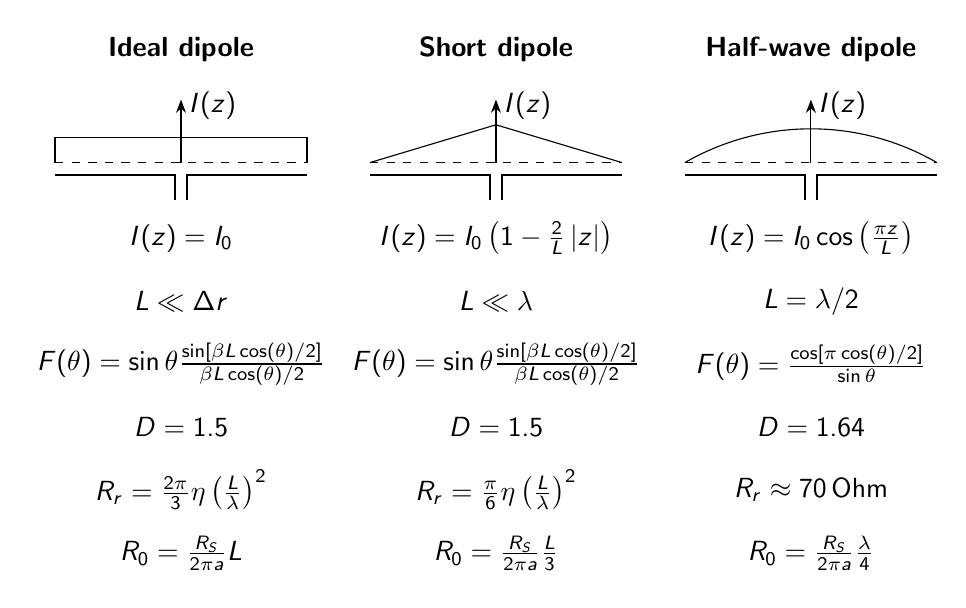
\begin{tikzpicture}[scale=0.8]
    %% Dipoles
    \foreach \x in {-5,0,5}
    {
    \draw[thick]
    (\x-2,0) to (\x-0.1,0) to (\x-0.1,-0.4)
    (\x+0.1,-0.4) to (\x+0.1,0) to (\x+2,0)
    ;
    
    \draw[-Stealth]
    (\x,0.2) to (\x,1.2)
    ;

    \draw[dashed]
    (\x-2,0.2) to (\x+2,0.2)
    ;
    
    \draw
    (\x+0.5,1.1) node{\(I(z)\)}
    ;
    }
    %% Ideal dipole
    \draw
    (-3,0.2) to (-3,0.6) to (-7,0.6) to (-7,0.2)
    ;
    \draw
    (-5,2) node{\textbf{Ideal dipole}}
    ;
    \draw
    (-5,-1) node{\(I(z) = I_0\)}
    (-5,-2) node{\(L \ll \Delta r\)}
    (-5,-3) node{\( F(\theta) = \sin \theta \frac{ \sin \left[ \beta L \cos ( \theta )/2 \right]}{ \beta L \cos ( \theta )/2} \)}
    (-5,-4) node{\(D=1.5\)}
    (-5,-5) node{\(R_r = \frac{2\pi}{3} \eta \left( \frac{L}{\lambda} \right)^2\)}
    (-5,-6) node{\(R_0 = \frac{R_S}{2\pi a} L\)}
    ;
    %% Short dipole
    \draw
    (2,0.2) to (0,0.8) to (-2,0.2)
    ;
    \draw
    (0,2) node{\textbf{Short dipole}}
    ;
    \draw
    (0,-1) node{\( I(z) = I_0 \left( 1 - \frac{2}{L} \left| z \right| \right) \)}
    (0,-2) node{\(L \ll \lambda\)}
    (0,-3) node{\( F(\theta) = \sin \theta \frac{ \sin \left[ \beta L \cos ( \theta )/2 \right]}{ \beta L \cos ( \theta )/2} \)}
    (0,-4) node{\(D=1.5\)}
    (0,-5) node{\(R_r = \frac{\pi}{6} \eta \left( \frac{L}{\lambda} \right)^2\)}
    (0,-6) node{\(R_0 = \frac{R_S}{2\pi a} \frac{L}{3}\)}
    ;
    %% Half-wavelenght antenna
    \draw
    (7,0.2) arc(60:120:4)
    ;
    \draw
    (5,2) node{\textbf{Half-wave dipole}}
    ;
    \draw
    (5,-1) node{\( I(z) = I_0 \cos \left( \frac{\pi z}{L} \right) \)}
    (5,-2) node{\(L = \lambda/2\)}
    (5,-3) node{\( F(\theta) = \frac{ \cos \left[ \pi \cos (\theta) /2 \right] }{\sin \theta} \)}
    (5,-4) node{\(D=1.64\)}
    (5,-5) node{\(R_r \approx \SI{70}{Ohm}\)}
    (5,-6) node{\(R_0 = \frac{R_S}{2\pi a} \frac{\lambda}{4}\)}
    ;
\end{tikzpicture}

\end{document}